% Created by tikzDevice version 0.12.3.1 on 2022-03-23 10:10:53
% !TEX encoding = UTF-8 Unicode
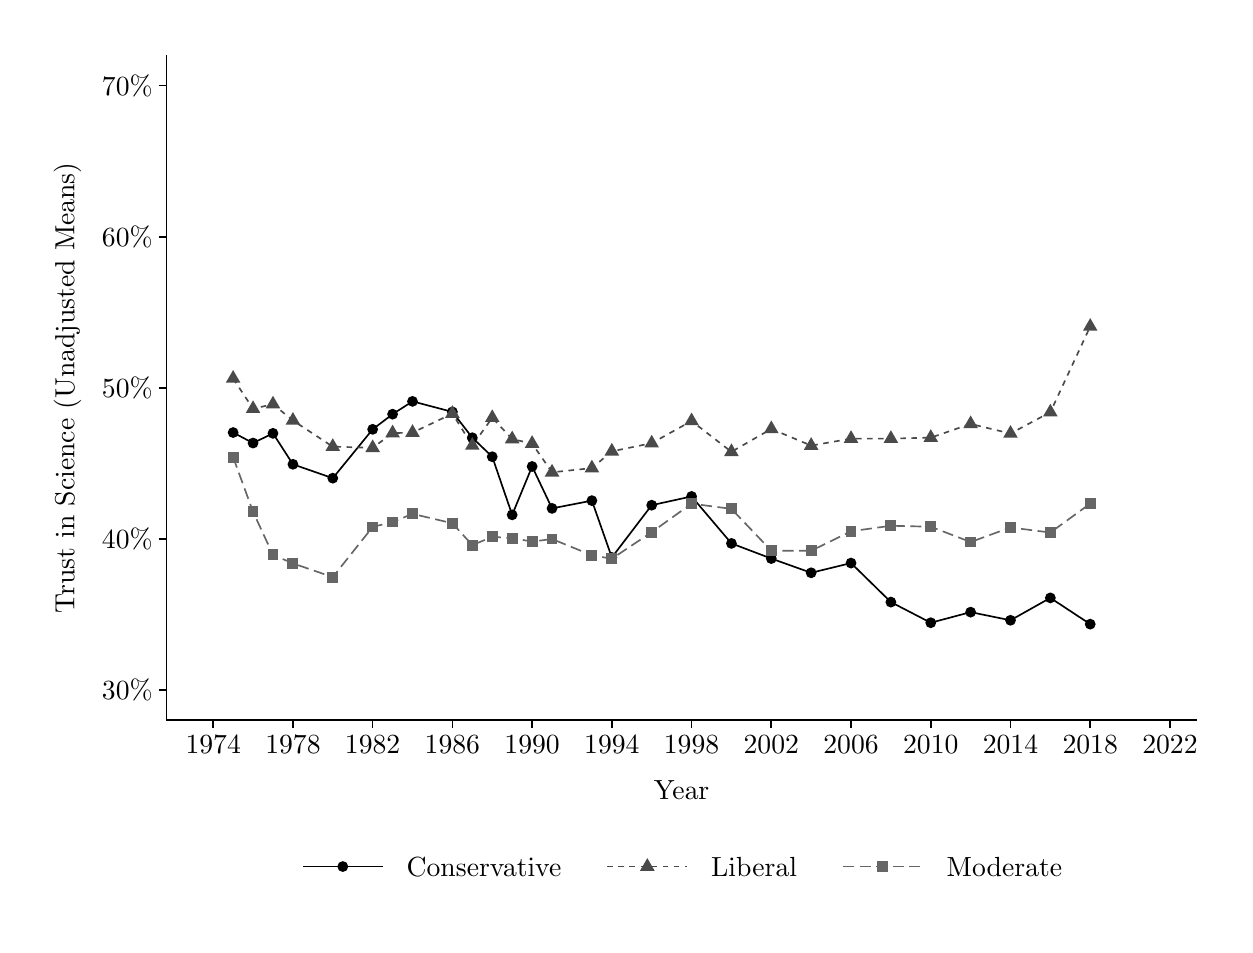
\begin{tikzpicture}[x=1pt,y=1pt]
\definecolor{fillColor}{RGB}{255,255,255}
\path[use as bounding box,fill=fillColor,fill opacity=0.00] (0,0) rectangle (432.48,324.36);
\begin{scope}
\path[clip] (  0.00,  0.00) rectangle (432.48,324.36);
\definecolor{fillColor}{RGB}{255,255,255}

\path[fill=fillColor] ( -0.00,  0.00) rectangle (432.48,324.36);
\end{scope}
\begin{scope}
\path[clip] ( 50.11, 74.07) rectangle (422.48,314.36);
\definecolor{fillColor}{RGB}{255,255,255}

\path[fill=fillColor] ( 50.11, 74.07) rectangle (422.48,314.36);
\definecolor{drawColor}{RGB}{0,0,0}

\path[draw=drawColor,line width= 0.6pt,line join=round] ( 74.24,178.06) --
	( 81.44,174.26) --
	( 88.64,177.77) --
	( 95.85,166.58) --
	(110.25,161.57) --
	(124.66,179.22) --
	(131.86,184.69) --
	(139.06,189.32) --
	(153.47,185.52) --
	(160.67,176.19) --
	(167.87,169.32) --
	(175.07,148.32) --
	(182.28,165.79) --
	(189.48,150.65) --
	(203.88,153.45) --
	(211.09,132.92) --
	(225.49,151.81) --
	(239.90,154.97) --
	(254.30,138.00) --
	(268.71,132.52) --
	(283.11,127.38) --
	(297.52,130.89) --
	(311.92,116.79) --
	(326.33,109.33) --
	(340.73,113.16) --
	(355.14,110.22) --
	(369.54,118.31) --
	(383.95,108.82);
\definecolor{drawColor}{gray}{0.29}

\path[draw=drawColor,line width= 0.6pt,dash pattern=on 2pt off 2pt ,line join=round] ( 74.24,197.60) --
	( 81.44,186.65) --
	( 88.64,188.30) --
	( 95.85,182.40) --
	(110.25,172.96) --
	(124.66,172.54) --
	(131.86,177.86) --
	(139.06,178.02) --
	(153.47,184.89) --
	(160.67,173.37) --
	(167.87,183.39) --
	(175.07,175.71) --
	(182.28,174.06) --
	(189.48,163.69) --
	(203.88,165.20) --
	(211.09,171.27) --
	(225.49,174.20) --
	(239.90,182.24) --
	(254.30,171.09) --
	(268.71,179.37) --
	(283.11,173.34) --
	(297.52,175.85) --
	(311.92,175.85) --
	(326.33,176.22) --
	(340.73,181.17) --
	(355.14,177.70) --
	(369.54,185.41) --
	(383.95,216.37);
\definecolor{drawColor}{gray}{0.40}

\path[draw=drawColor,line width= 0.6pt,dash pattern=on 4pt off 2pt ,line join=round] ( 74.24,169.16) --
	( 81.44,149.41) --
	( 88.64,133.86) --
	( 95.85,130.78) --
	(110.25,125.82) --
	(124.66,143.95) --
	(131.86,145.72) --
	(139.06,148.67) --
	(153.47,145.28) --
	(160.67,137.37) --
	(167.87,140.37) --
	(175.07,139.92) --
	(182.28,138.65) --
	(189.48,139.58) --
	(203.88,133.71) --
	(211.09,132.46) --
	(225.49,142.07) --
	(239.90,152.37) --
	(254.30,150.48) --
	(268.71,135.36) --
	(283.11,135.33) --
	(297.52,142.39) --
	(311.92,144.37) --
	(326.33,144.03) --
	(340.73,138.49) --
	(355.14,143.76) --
	(369.54,141.92) --
	(383.95,152.38);
\definecolor{fillColor}{RGB}{0,0,0}

\path[fill=fillColor] ( 74.24,178.06) circle (  1.96);
\definecolor{fillColor}{gray}{0.29}

\path[fill=fillColor] ( 74.24,200.65) --
	( 76.88,196.08) --
	( 71.60,196.08) --
	cycle;
\definecolor{fillColor}{gray}{0.40}

\path[fill=fillColor] ( 72.28,167.20) --
	( 76.20,167.20) --
	( 76.20,171.12) --
	( 72.28,171.12) --
	cycle;
\definecolor{fillColor}{RGB}{0,0,0}

\path[fill=fillColor] ( 81.44,174.26) circle (  1.96);
\definecolor{fillColor}{gray}{0.29}

\path[fill=fillColor] ( 81.44,189.70) --
	( 84.08,185.12) --
	( 78.80,185.12) --
	cycle;
\definecolor{fillColor}{gray}{0.40}

\path[fill=fillColor] ( 79.48,147.44) --
	( 83.40,147.44) --
	( 83.40,151.37) --
	( 79.48,151.37) --
	cycle;
\definecolor{fillColor}{RGB}{0,0,0}

\path[fill=fillColor] ( 88.64,177.77) circle (  1.96);
\definecolor{fillColor}{gray}{0.29}

\path[fill=fillColor] ( 88.64,191.35) --
	( 91.29,186.77) --
	( 86.00,186.77) --
	cycle;
\definecolor{fillColor}{gray}{0.40}

\path[fill=fillColor] ( 86.68,131.90) --
	( 90.61,131.90) --
	( 90.61,135.82) --
	( 86.68,135.82) --
	cycle;
\definecolor{fillColor}{RGB}{0,0,0}

\path[fill=fillColor] ( 95.85,166.58) circle (  1.96);
\definecolor{fillColor}{gray}{0.29}

\path[fill=fillColor] ( 95.85,185.46) --
	( 98.49,180.88) --
	( 93.20,180.88) --
	cycle;
\definecolor{fillColor}{gray}{0.40}

\path[fill=fillColor] ( 93.88,128.82) --
	( 97.81,128.82) --
	( 97.81,132.74) --
	( 93.88,132.74) --
	cycle;
\definecolor{fillColor}{RGB}{0,0,0}

\path[fill=fillColor] (110.25,161.57) circle (  1.96);
\definecolor{fillColor}{gray}{0.29}

\path[fill=fillColor] (110.25,176.01) --
	(112.89,171.43) --
	(107.61,171.43) --
	cycle;
\definecolor{fillColor}{gray}{0.40}

\path[fill=fillColor] (108.29,123.86) --
	(112.21,123.86) --
	(112.21,127.79) --
	(108.29,127.79) --
	cycle;
\definecolor{fillColor}{RGB}{0,0,0}

\path[fill=fillColor] (124.66,179.22) circle (  1.96);
\definecolor{fillColor}{gray}{0.29}

\path[fill=fillColor] (124.66,175.59) --
	(127.30,171.01) --
	(122.01,171.01) --
	cycle;
\definecolor{fillColor}{gray}{0.40}

\path[fill=fillColor] (122.69,141.99) --
	(126.62,141.99) --
	(126.62,145.91) --
	(122.69,145.91) --
	cycle;
\definecolor{fillColor}{RGB}{0,0,0}

\path[fill=fillColor] (131.86,184.69) circle (  1.96);
\definecolor{fillColor}{gray}{0.29}

\path[fill=fillColor] (131.86,180.91) --
	(134.50,176.33) --
	(129.22,176.33) --
	cycle;
\definecolor{fillColor}{gray}{0.40}

\path[fill=fillColor] (129.90,143.76) --
	(133.82,143.76) --
	(133.82,147.68) --
	(129.90,147.68) --
	cycle;
\definecolor{fillColor}{RGB}{0,0,0}

\path[fill=fillColor] (139.06,189.32) circle (  1.96);
\definecolor{fillColor}{gray}{0.29}

\path[fill=fillColor] (139.06,181.07) --
	(141.70,176.49) --
	(136.42,176.49) --
	cycle;
\definecolor{fillColor}{gray}{0.40}

\path[fill=fillColor] (137.10,146.71) --
	(141.02,146.71) --
	(141.02,150.63) --
	(137.10,150.63) --
	cycle;
\definecolor{fillColor}{RGB}{0,0,0}

\path[fill=fillColor] (153.47,185.52) circle (  1.96);
\definecolor{fillColor}{gray}{0.29}

\path[fill=fillColor] (153.47,187.95) --
	(156.11,183.37) --
	(150.82,183.37) --
	cycle;
\definecolor{fillColor}{gray}{0.40}

\path[fill=fillColor] (151.50,143.31) --
	(155.43,143.31) --
	(155.43,147.24) --
	(151.50,147.24) --
	cycle;
\definecolor{fillColor}{RGB}{0,0,0}

\path[fill=fillColor] (160.67,176.19) circle (  1.96);
\definecolor{fillColor}{gray}{0.29}

\path[fill=fillColor] (160.67,176.42) --
	(163.31,171.84) --
	(158.03,171.84) --
	cycle;
\definecolor{fillColor}{gray}{0.40}

\path[fill=fillColor] (158.71,135.41) --
	(162.63,135.41) --
	(162.63,139.34) --
	(158.71,139.34) --
	cycle;
\definecolor{fillColor}{RGB}{0,0,0}

\path[fill=fillColor] (167.87,169.32) circle (  1.96);
\definecolor{fillColor}{gray}{0.29}

\path[fill=fillColor] (167.87,186.45) --
	(170.51,181.87) --
	(165.23,181.87) --
	cycle;
\definecolor{fillColor}{gray}{0.40}

\path[fill=fillColor] (165.91,138.41) --
	(169.83,138.41) --
	(169.83,142.33) --
	(165.91,142.33) --
	cycle;
\definecolor{fillColor}{RGB}{0,0,0}

\path[fill=fillColor] (175.07,148.32) circle (  1.96);
\definecolor{fillColor}{gray}{0.29}

\path[fill=fillColor] (175.07,178.76) --
	(177.72,174.18) --
	(172.43,174.18) --
	cycle;
\definecolor{fillColor}{gray}{0.40}

\path[fill=fillColor] (173.11,137.96) --
	(177.04,137.96) --
	(177.04,141.88) --
	(173.11,141.88) --
	cycle;
\definecolor{fillColor}{RGB}{0,0,0}

\path[fill=fillColor] (182.28,165.79) circle (  1.96);
\definecolor{fillColor}{gray}{0.29}

\path[fill=fillColor] (182.28,177.11) --
	(184.92,172.54) --
	(179.63,172.54) --
	cycle;
\definecolor{fillColor}{gray}{0.40}

\path[fill=fillColor] (180.31,136.69) --
	(184.24,136.69) --
	(184.24,140.61) --
	(180.31,140.61) --
	cycle;
\definecolor{fillColor}{RGB}{0,0,0}

\path[fill=fillColor] (189.48,150.65) circle (  1.96);
\definecolor{fillColor}{gray}{0.29}

\path[fill=fillColor] (189.48,166.74) --
	(192.12,162.17) --
	(186.84,162.17) --
	cycle;
\definecolor{fillColor}{gray}{0.40}

\path[fill=fillColor] (187.52,137.62) --
	(191.44,137.62) --
	(191.44,141.55) --
	(187.52,141.55) --
	cycle;
\definecolor{fillColor}{RGB}{0,0,0}

\path[fill=fillColor] (203.88,153.45) circle (  1.96);
\definecolor{fillColor}{gray}{0.29}

\path[fill=fillColor] (203.88,168.25) --
	(206.53,163.67) --
	(201.24,163.67) --
	cycle;
\definecolor{fillColor}{gray}{0.40}

\path[fill=fillColor] (201.92,131.75) --
	(205.85,131.75) --
	(205.85,135.68) --
	(201.92,135.68) --
	cycle;
\definecolor{fillColor}{RGB}{0,0,0}

\path[fill=fillColor] (211.09,132.92) circle (  1.96);
\definecolor{fillColor}{gray}{0.29}

\path[fill=fillColor] (211.09,174.32) --
	(213.73,169.74) --
	(208.44,169.74) --
	cycle;
\definecolor{fillColor}{gray}{0.40}

\path[fill=fillColor] (209.12,130.49) --
	(213.05,130.49) --
	(213.05,134.42) --
	(209.12,134.42) --
	cycle;
\definecolor{fillColor}{RGB}{0,0,0}

\path[fill=fillColor] (225.49,151.81) circle (  1.96);
\definecolor{fillColor}{gray}{0.29}

\path[fill=fillColor] (225.49,177.25) --
	(228.13,172.67) --
	(222.85,172.67) --
	cycle;
\definecolor{fillColor}{gray}{0.40}

\path[fill=fillColor] (223.53,140.11) --
	(227.45,140.11) --
	(227.45,144.03) --
	(223.53,144.03) --
	cycle;
\definecolor{fillColor}{RGB}{0,0,0}

\path[fill=fillColor] (239.90,154.97) circle (  1.96);
\definecolor{fillColor}{gray}{0.29}

\path[fill=fillColor] (239.90,185.29) --
	(242.54,180.72) --
	(237.25,180.72) --
	cycle;
\definecolor{fillColor}{gray}{0.40}

\path[fill=fillColor] (237.94,150.41) --
	(241.86,150.41) --
	(241.86,154.33) --
	(237.94,154.33) --
	cycle;
\definecolor{fillColor}{RGB}{0,0,0}

\path[fill=fillColor] (254.30,138.00) circle (  1.96);
\definecolor{fillColor}{gray}{0.29}

\path[fill=fillColor] (254.30,174.14) --
	(256.94,169.56) --
	(251.66,169.56) --
	cycle;
\definecolor{fillColor}{gray}{0.40}

\path[fill=fillColor] (252.34,148.51) --
	(256.26,148.51) --
	(256.26,152.44) --
	(252.34,152.44) --
	cycle;
\definecolor{fillColor}{RGB}{0,0,0}

\path[fill=fillColor] (268.71,132.52) circle (  1.96);
\definecolor{fillColor}{gray}{0.29}

\path[fill=fillColor] (268.71,182.42) --
	(271.35,177.84) --
	(266.06,177.84) --
	cycle;
\definecolor{fillColor}{gray}{0.40}

\path[fill=fillColor] (266.75,133.40) --
	(270.67,133.40) --
	(270.67,137.32) --
	(266.75,137.32) --
	cycle;
\definecolor{fillColor}{RGB}{0,0,0}

\path[fill=fillColor] (283.11,127.38) circle (  1.96);
\definecolor{fillColor}{gray}{0.29}

\path[fill=fillColor] (283.11,176.39) --
	(285.76,171.81) --
	(280.47,171.81) --
	cycle;
\definecolor{fillColor}{gray}{0.40}

\path[fill=fillColor] (281.15,133.37) --
	(285.07,133.37) --
	(285.07,137.29) --
	(281.15,137.29) --
	cycle;
\definecolor{fillColor}{RGB}{0,0,0}

\path[fill=fillColor] (297.52,130.89) circle (  1.96);
\definecolor{fillColor}{gray}{0.29}

\path[fill=fillColor] (297.52,178.90) --
	(300.16,174.32) --
	(294.88,174.32) --
	cycle;
\definecolor{fillColor}{gray}{0.40}

\path[fill=fillColor] (295.56,140.43) --
	(299.48,140.43) --
	(299.48,144.35) --
	(295.56,144.35) --
	cycle;
\definecolor{fillColor}{RGB}{0,0,0}

\path[fill=fillColor] (311.92,116.79) circle (  1.96);
\definecolor{fillColor}{gray}{0.29}

\path[fill=fillColor] (311.92,178.90) --
	(314.57,174.33) --
	(309.28,174.33) --
	cycle;
\definecolor{fillColor}{gray}{0.40}

\path[fill=fillColor] (309.96,142.40) --
	(313.88,142.40) --
	(313.88,146.33) --
	(309.96,146.33) --
	cycle;
\definecolor{fillColor}{RGB}{0,0,0}

\path[fill=fillColor] (326.33,109.33) circle (  1.96);
\definecolor{fillColor}{gray}{0.29}

\path[fill=fillColor] (326.33,179.27) --
	(328.97,174.69) --
	(323.69,174.69) --
	cycle;
\definecolor{fillColor}{gray}{0.40}

\path[fill=fillColor] (324.37,142.07) --
	(328.29,142.07) --
	(328.29,145.99) --
	(324.37,145.99) --
	cycle;
\definecolor{fillColor}{RGB}{0,0,0}

\path[fill=fillColor] (340.73,113.16) circle (  1.96);
\definecolor{fillColor}{gray}{0.29}

\path[fill=fillColor] (340.73,184.23) --
	(343.38,179.65) --
	(338.09,179.65) --
	cycle;
\definecolor{fillColor}{gray}{0.40}

\path[fill=fillColor] (338.77,136.52) --
	(342.70,136.52) --
	(342.70,140.45) --
	(338.77,140.45) --
	cycle;
\definecolor{fillColor}{RGB}{0,0,0}

\path[fill=fillColor] (355.14,110.22) circle (  1.96);
\definecolor{fillColor}{gray}{0.29}

\path[fill=fillColor] (355.14,180.76) --
	(357.78,176.18) --
	(352.50,176.18) --
	cycle;
\definecolor{fillColor}{gray}{0.40}

\path[fill=fillColor] (353.18,141.79) --
	(357.10,141.79) --
	(357.10,145.72) --
	(353.18,145.72) --
	cycle;
\definecolor{fillColor}{RGB}{0,0,0}

\path[fill=fillColor] (369.54,118.31) circle (  1.96);
\definecolor{fillColor}{gray}{0.29}

\path[fill=fillColor] (369.54,188.46) --
	(372.19,183.88) --
	(366.90,183.88) --
	cycle;
\definecolor{fillColor}{gray}{0.40}

\path[fill=fillColor] (367.58,139.96) --
	(371.51,139.96) --
	(371.51,143.88) --
	(367.58,143.88) --
	cycle;
\definecolor{fillColor}{RGB}{0,0,0}

\path[fill=fillColor] (383.95,108.82) circle (  1.96);
\definecolor{fillColor}{gray}{0.29}

\path[fill=fillColor] (383.95,219.42) --
	(386.59,214.84) --
	(381.31,214.84) --
	cycle;
\definecolor{fillColor}{gray}{0.40}

\path[fill=fillColor] (381.99,150.42) --
	(385.91,150.42) --
	(385.91,154.35) --
	(381.99,154.35) --
	cycle;
\end{scope}
\begin{scope}
\path[clip] (  0.00,  0.00) rectangle (432.48,324.36);
\definecolor{drawColor}{RGB}{0,0,0}

\path[draw=drawColor,line width= 0.6pt,line join=round] ( 50.11, 74.07) --
	( 50.11,314.36);
\end{scope}
\begin{scope}
\path[clip] (  0.00,  0.00) rectangle (432.48,324.36);
\definecolor{drawColor}{RGB}{0,0,0}

\node[text=drawColor,anchor=base east,inner sep=0pt, outer sep=0pt, scale=  1.00] at ( 45.16, 81.55) {30{\%}};

\node[text=drawColor,anchor=base east,inner sep=0pt, outer sep=0pt, scale=  1.00] at ( 45.16,136.16) {40{\%}};

\node[text=drawColor,anchor=base east,inner sep=0pt, outer sep=0pt, scale=  1.00] at ( 45.16,190.77) {50{\%}};

\node[text=drawColor,anchor=base east,inner sep=0pt, outer sep=0pt, scale=  1.00] at ( 45.16,245.38) {60{\%}};

\node[text=drawColor,anchor=base east,inner sep=0pt, outer sep=0pt, scale=  1.00] at ( 45.16,300.00) {70{\%}};
\end{scope}
\begin{scope}
\path[clip] (  0.00,  0.00) rectangle (432.48,324.36);
\definecolor{drawColor}{RGB}{0,0,0}

\path[draw=drawColor,line width= 0.6pt,line join=round] ( 47.36, 84.99) --
	( 50.11, 84.99);

\path[draw=drawColor,line width= 0.6pt,line join=round] ( 47.36,139.60) --
	( 50.11,139.60);

\path[draw=drawColor,line width= 0.6pt,line join=round] ( 47.36,194.21) --
	( 50.11,194.21);

\path[draw=drawColor,line width= 0.6pt,line join=round] ( 47.36,248.83) --
	( 50.11,248.83);

\path[draw=drawColor,line width= 0.6pt,line join=round] ( 47.36,303.44) --
	( 50.11,303.44);
\end{scope}
\begin{scope}
\path[clip] (  0.00,  0.00) rectangle (432.48,324.36);
\definecolor{drawColor}{RGB}{0,0,0}

\path[draw=drawColor,line width= 0.6pt,line join=round] ( 50.11, 74.07) --
	(422.48, 74.07);
\end{scope}
\begin{scope}
\path[clip] (  0.00,  0.00) rectangle (432.48,324.36);
\definecolor{drawColor}{RGB}{0,0,0}

\path[draw=drawColor,line width= 0.6pt,line join=round] ( 67.04, 71.32) --
	( 67.04, 74.07);

\path[draw=drawColor,line width= 0.6pt,line join=round] ( 95.85, 71.32) --
	( 95.85, 74.07);

\path[draw=drawColor,line width= 0.6pt,line join=round] (124.66, 71.32) --
	(124.66, 74.07);

\path[draw=drawColor,line width= 0.6pt,line join=round] (153.47, 71.32) --
	(153.47, 74.07);

\path[draw=drawColor,line width= 0.6pt,line join=round] (182.28, 71.32) --
	(182.28, 74.07);

\path[draw=drawColor,line width= 0.6pt,line join=round] (211.09, 71.32) --
	(211.09, 74.07);

\path[draw=drawColor,line width= 0.6pt,line join=round] (239.90, 71.32) --
	(239.90, 74.07);

\path[draw=drawColor,line width= 0.6pt,line join=round] (268.71, 71.32) --
	(268.71, 74.07);

\path[draw=drawColor,line width= 0.6pt,line join=round] (297.52, 71.32) --
	(297.52, 74.07);

\path[draw=drawColor,line width= 0.6pt,line join=round] (326.33, 71.32) --
	(326.33, 74.07);

\path[draw=drawColor,line width= 0.6pt,line join=round] (355.14, 71.32) --
	(355.14, 74.07);

\path[draw=drawColor,line width= 0.6pt,line join=round] (383.95, 71.32) --
	(383.95, 74.07);

\path[draw=drawColor,line width= 0.6pt,line join=round] (412.76, 71.32) --
	(412.76, 74.07);
\end{scope}
\begin{scope}
\path[clip] (  0.00,  0.00) rectangle (432.48,324.36);
\definecolor{drawColor}{RGB}{0,0,0}

\node[text=drawColor,anchor=base,inner sep=0pt, outer sep=0pt, scale=  1.00] at ( 67.04, 62.23) {1974};

\node[text=drawColor,anchor=base,inner sep=0pt, outer sep=0pt, scale=  1.00] at ( 95.85, 62.23) {1978};

\node[text=drawColor,anchor=base,inner sep=0pt, outer sep=0pt, scale=  1.00] at (124.66, 62.23) {1982};

\node[text=drawColor,anchor=base,inner sep=0pt, outer sep=0pt, scale=  1.00] at (153.47, 62.23) {1986};

\node[text=drawColor,anchor=base,inner sep=0pt, outer sep=0pt, scale=  1.00] at (182.28, 62.23) {1990};

\node[text=drawColor,anchor=base,inner sep=0pt, outer sep=0pt, scale=  1.00] at (211.09, 62.23) {1994};

\node[text=drawColor,anchor=base,inner sep=0pt, outer sep=0pt, scale=  1.00] at (239.90, 62.23) {1998};

\node[text=drawColor,anchor=base,inner sep=0pt, outer sep=0pt, scale=  1.00] at (268.71, 62.23) {2002};

\node[text=drawColor,anchor=base,inner sep=0pt, outer sep=0pt, scale=  1.00] at (297.52, 62.23) {2006};

\node[text=drawColor,anchor=base,inner sep=0pt, outer sep=0pt, scale=  1.00] at (326.33, 62.23) {2010};

\node[text=drawColor,anchor=base,inner sep=0pt, outer sep=0pt, scale=  1.00] at (355.14, 62.23) {2014};

\node[text=drawColor,anchor=base,inner sep=0pt, outer sep=0pt, scale=  1.00] at (383.95, 62.23) {2018};

\node[text=drawColor,anchor=base,inner sep=0pt, outer sep=0pt, scale=  1.00] at (412.76, 62.23) {2022};
\end{scope}
\begin{scope}
\path[clip] (  0.00,  0.00) rectangle (432.48,324.36);
\definecolor{drawColor}{RGB}{0,0,0}

\node[text=drawColor,anchor=base,inner sep=0pt, outer sep=0pt, scale=  1.00] at (236.30, 45.40) {Year};
\end{scope}
\begin{scope}
\path[clip] (  0.00,  0.00) rectangle (432.48,324.36);
\definecolor{drawColor}{RGB}{0,0,0}

\node[text=drawColor,rotate= 90.00,anchor=base,inner sep=0pt, outer sep=0pt, scale=  1.00] at ( 16.89,194.21) {Trust in Science (Unadjusted Means)};
\end{scope}
\begin{scope}
\path[clip] (  0.00,  0.00) rectangle (432.48,324.36);

\path[] ( 86.80, 10.00) rectangle (385.79, 32.45);
\end{scope}
\begin{scope}
\path[clip] (  0.00,  0.00) rectangle (432.48,324.36);

\path[] ( 95.80, 14.00) rectangle (131.94, 28.45);
\end{scope}
\begin{scope}
\path[clip] (  0.00,  0.00) rectangle (432.48,324.36);
\definecolor{drawColor}{RGB}{0,0,0}

\path[draw=drawColor,line width= 0.6pt,line join=round] ( 99.42, 21.23) -- (128.33, 21.23);
\end{scope}
\begin{scope}
\path[clip] (  0.00,  0.00) rectangle (432.48,324.36);
\definecolor{fillColor}{RGB}{0,0,0}

\path[fill=fillColor] (113.87, 21.23) circle (  1.96);
\end{scope}
\begin{scope}
\path[clip] (  0.00,  0.00) rectangle (432.48,324.36);

\path[] (205.84, 14.00) rectangle (241.98, 28.45);
\end{scope}
\begin{scope}
\path[clip] (  0.00,  0.00) rectangle (432.48,324.36);
\definecolor{drawColor}{gray}{0.29}

\path[draw=drawColor,line width= 0.6pt,dash pattern=on 2pt off 2pt ,line join=round] (209.46, 21.23) -- (238.36, 21.23);
\end{scope}
\begin{scope}
\path[clip] (  0.00,  0.00) rectangle (432.48,324.36);
\definecolor{fillColor}{gray}{0.29}

\path[fill=fillColor] (223.91, 24.28) --
	(226.55, 19.70) --
	(221.27, 19.70) --
	cycle;
\end{scope}
\begin{scope}
\path[clip] (  0.00,  0.00) rectangle (432.48,324.36);

\path[] (290.97, 14.00) rectangle (327.10, 28.45);
\end{scope}
\begin{scope}
\path[clip] (  0.00,  0.00) rectangle (432.48,324.36);
\definecolor{drawColor}{gray}{0.40}

\path[draw=drawColor,line width= 0.6pt,dash pattern=on 4pt off 2pt ,line join=round] (294.58, 21.23) -- (323.49, 21.23);
\end{scope}
\begin{scope}
\path[clip] (  0.00,  0.00) rectangle (432.48,324.36);
\definecolor{fillColor}{gray}{0.40}

\path[fill=fillColor] (307.07, 19.26) --
	(311.00, 19.26) --
	(311.00, 23.19) --
	(307.07, 23.19) --
	cycle;
\end{scope}
\begin{scope}
\path[clip] (  0.00,  0.00) rectangle (432.48,324.36);
\definecolor{drawColor}{RGB}{0,0,0}

\node[text=drawColor,anchor=base west,inner sep=0pt, outer sep=0pt, scale=  1.00] at (136.94, 17.78) {Conservative};
\end{scope}
\begin{scope}
\path[clip] (  0.00,  0.00) rectangle (432.48,324.36);
\definecolor{drawColor}{RGB}{0,0,0}

\node[text=drawColor,anchor=base west,inner sep=0pt, outer sep=0pt, scale=  1.00] at (246.98, 17.78) {Liberal};
\end{scope}
\begin{scope}
\path[clip] (  0.00,  0.00) rectangle (432.48,324.36);
\definecolor{drawColor}{RGB}{0,0,0}

\node[text=drawColor,anchor=base west,inner sep=0pt, outer sep=0pt, scale=  1.00] at (332.10, 17.78) {Moderate};
\end{scope}
\end{tikzpicture}
